\section{The limit of vanishing resolution}\label{ch:weak}

Neither closure under weak limits nor Bondesson's theorem reaches RH.

\subsection{Weak limits of Thorin measures}\label{sec:weak:limits}

\begin{theorem}[Thorin \cite{Thorin77a,Thorin}; Bondesson {\cite[Theorem 3.1.5]{Bondesson}}; see also {\cite[Theorem 18.9]{P26}}]
The class of GGC laws is closed under convergence in law.
\end{theorem}



\begin{corollary}\label{cor:weak:closure}
RH holds if and only if there are GGC variables $X_N$ with $\E e^{-uX_N}\to1/G(u)$ for all $u$ in a set with an accumulation point in $(0,\infty)$ \cite[Propositions 18.10 and 18.14]{P26}.
\end{corollary}

\begin{proof}
The transforms are analytic and bounded by one on $\re u>0$, so by Vitali's theorem they converge locally uniformly there, and the limit is $1/G$ on $(0,\infty)$. Since $1/G(u)\to1$ as $u\downarrow0$, the $X_N$ converge in law to a proper limit with transform $1/G$, which is a GGC by the closure theorem, and Proposition~\ref{prop:rigid} gives RH. Conversely, under RH the clock variable $T$ is a GGC with transform $1/G$; take $X_N=T$.
\end{proof}

The Cauchy flow $\varepsilon\mapsto\rho_\varepsilon$ of Section~\ref{ch:clock} is the candidate at hand. Its measures $\mu_\varepsilon$ are the Thorin measures of $\xi(\alpha)/\xi(\alpha+\sqrt u)$ at $\alpha=\tfrac12+\varepsilon$ whenever these are GGC transforms (Theorem~\ref{thm:poisson}), the transforms converge to $1/G$ pointwise as $\varepsilon\downarrow0$, and the measures converge vaguely. The flow fails for two reasons.

First, the limit is the wrong measure. As shown after Proposition~\ref{prop:struct}, $\mu_\varepsilon\to U_{\rm line}$ vaguely whatever the truth of RH \cite[Proposition 9.5]{P17}, because the contribution of an off line pair tends to zero in total variation (Proposition~\ref{prop:signature}(ii)); the limit omits the off line zeros. It is the Thorin measure of the clock only under RH, since the Thorin functional $U$ of Section~\ref{ch:arith} counts every zero and $U=U_{\rm line}$ exactly when RH holds (Section~\ref{sec:ch14:functional} and \cite[Proposition 7.6]{P26}). Positivity of the vague limit therefore carries no information.

Second, the closure theorem needs GGC laws along the sequence. The flow supplies a law at every resolution with no hypothesis, that of the shifted clock $T_\alpha$ of Theorem~\ref{bp:thm:alpha} at $\alpha=\tfrac12+\varepsilon$, but at small $\varepsilon$ it supplies a GGC law only under the hypothesis to be proved: the transform at basepoint $\tfrac12+\varepsilon$ is a GGC transform if and only if no zero lies to the right of the line $\re s=\tfrac12+\varepsilon$ (Theorem~\ref{thm:poisson}). Positivity of $\rho_\varepsilon$ at that one $\varepsilon$ is necessary for this but is not known to imply it, since near a cluster of line zeros the negative kernel of an off line pair can be outweighed by the kernels of its neighbours (Exercise~\ref{ex:ch2:line} and Section~\ref{sec:ch13:visibility}). Positivity of $\rho_{\varepsilon'}$ for every $\varepsilon'>\varepsilon$ does imply it, as shown in Remark~\ref{rem:ch2:oneline}; for $\varepsilon=0$ this is Lagarias's criterion \cite{Lagarias}, which is RH. Weak closure adds the endpoint $\varepsilon=0$ to a family already known to consist of GGCs; it cannot show that the family consists of GGCs \cite[Remark 3.10]{P26}.

On the window $0\le\theta\le200$ the P\'olya route computes $\min\rho_\varepsilon=0.0147\,\varepsilon>0$ at each of the eight resolutions of Table~\ref{tab:tv}, down to $\varepsilon=0.005$ (Section~\ref{sec:ch6:measure}); with the verification of RH to height $3\times10^{12}$ this is a theorem, since for every $\varepsilon\le6.85$ the minimum of $\rho_\varepsilon$ over $[0,3\times10^{12}-1.21]$ is $\rho_\varepsilon(0)$ (Theorem~\ref{thm:dbeta:minall} and Remark~\ref{rem:dbeta:margin}), and Section~\ref{st:sec:wp2} lists what would make the P\'olya computation itself a certificate.

Weak convergence becomes useful only with approximants whose positivity is proved independently of $\xi$, such as Beurling generalised prime systems whose zeta functions provably have only real ordinates, finite Krein strings, and the partial products over verified zeros completed by the Weyl tail; the last two are the Kent approximants of Section~\ref{sec:ch18:kent}, without and with the Weyl tail. For such approximants the distances of Section~\ref{ch:distances} are the right measure of the approximation. Verification also removes factors from the question: if the first $N$ zeros are verified to lie on the line, then $1/G_N$, with $G_N(u)=\prod_{k\le N}(1+u/\gamma_k^2)$, is a GGC transform with no hypothesis, and RH holds if and only if the tail factor $G_N/G$ is a GGC transform as well \cite[Corollary 18.11]{P26}.


\subsection{The HCM form of the Thorin condition}\label{sec:weak:hcm}

Bondesson's theorem (Section~\ref{sec:ch3:hierarchy}; \cite[Theorem 6.1.1]{Bondesson}, see also \cite{JRY}) and the results of Section~\ref{ch:clock} give the following.

\begin{corollary}\label{cor:hcm}
(i) For every $\alpha\ge1$ the function $\varphi_\alpha(u)=\xi(\alpha)/\xi(\alpha+\sqrt u)$ is HCM, unconditionally. (ii) The reciprocal Xi function $\varphi_{1/2}(u)=\xi(\tfrac12)/\xi(\tfrac12+\sqrt u)$, which is the clock $1/G$, is HCM if and only if RH holds.
\end{corollary}

\begin{proof}
(i) is Theorem~\ref{thm:poisson} with Bondesson's theorem, and (ii) is Proposition~\ref{prop:rigid} with Bondesson's theorem.
\end{proof}



By the Hadamard product \eqref{eq:ch2:hadamard}, with $a_k=-(\rho_k-\tfrac12)^2$ and $w=v+1/v$,
\begin{equation}\label{eq:hcmprod}
\varphi_{1/2}(uv)\,\varphi_{1/2}(u/v)=\prod_k\frac{a_k^2}{a_k^2+a_k\,u\,w+u^2}=\prod_k\frac{a_k/u}{w+c_k(u)},\qquad c_k(u)=\frac{a_k}{u}+\frac{u}{a_k}.
\end{equation}
The numbers $c_k(u)$ are local to this subsection, and are not the derivatives $c_k(t)$ of the heat trace in Section~\ref{ch:heat}. An off line pair, with values $a$ and $\bar a$ of $a_k$, contributes $(|a|^2/u^2)/((w+c)(w+\bar c))$ with $c=c(u)$ complex, and $1/((w+c)(w+\bar c))$ is the Laplace transform of the signed function $e^{-t\re c}\sin(t\im c)/\im c$. At a single $u$ the remaining factors may smooth this to a positive function; failure is guaranteed only across all $u$, by Bondesson's theorem. At $u=|a|$ both values of $c$ equal $2\cos\arg a$, and the pair contributes $(w+2\cos\arg a)^{-2}$, which is completely monotone on $[2,\infty)$. Complete monotonicity in $w$ at finitely many $u$ is therefore necessary for HCM but not sufficient.

We test this necessary condition. From $60$ digit values of $\xi$ at real arguments, computed by \eqref{eq:xi} without cancellation, numerical differentiation gives the normalised derivatives $d_k=(-1)^k\partial_w^kH_u(w)/H_u(w)$ of $H_u(w)=\varphi_\alpha(uv)\,\varphi_\alpha(u/v)$ for $k\le6$, $u\in\{1,25,400\}$ and $w\in\{2.05,3,5,10,20,50\}$, at $\alpha=\tfrac12$ and at the control $\alpha=1$. All $216$ values are positive (Figure~\ref{fig:hcm} shows $w=3$ and $w=20$), and the signs are certified: from the Taylor coefficients of $H_u$ in $w$, computed in ball arithmetic \cite{Arb} from $\xi(s)=\frac12s(s-1)\pi^{-s/2}\Gamma(\frac s2)\zeta(s)$, and so independently of the P\'olya route, every $d_k$ is enclosed in a ball of relative radius below $10^{-70}$ that lies in $(0,\infty)$. Under RH, \eqref{eq:hcmprod} gives $H_u(w+t)/H_u(w)=\E e^{-tY}$ with $Y=\sum_ke_k/(w+c_k(u))$ and independent standard exponentials $e_k$, so $d_k=\E Y^k$ is of order $d_1^k$. The smallest value, $2.5\times10^{-10}$ at $\alpha=\tfrac12$, $u=1$, $w=50$, $k=6$, is $2.54\,d_1^6$ with $d_1=0.0215$: it reflects the scale of $Y$, to which many zeros contribute, not closeness to a sign change. The test is consistent with (ii) and cannot decide it (Section~\ref{ch:finite}, Table~\ref{tab:ch13:see}, and \cite[Chapter 11]{P26}).

Under RH the clock variable is $T=\sum_{\gamma>0}e_\gamma/\gamma^2$ (Proposition~\ref{prop:rigid}), and if moreover the zeros are simple and satisfy two further hypotheses, its density is not HCM (Theorem~\ref{bs:thm:nb}); for the Cauchy analogue of the clock variable this holds unconditionally (Theorem~\ref{bs:thm:eta}).

\begin{figure}[t]
\centering
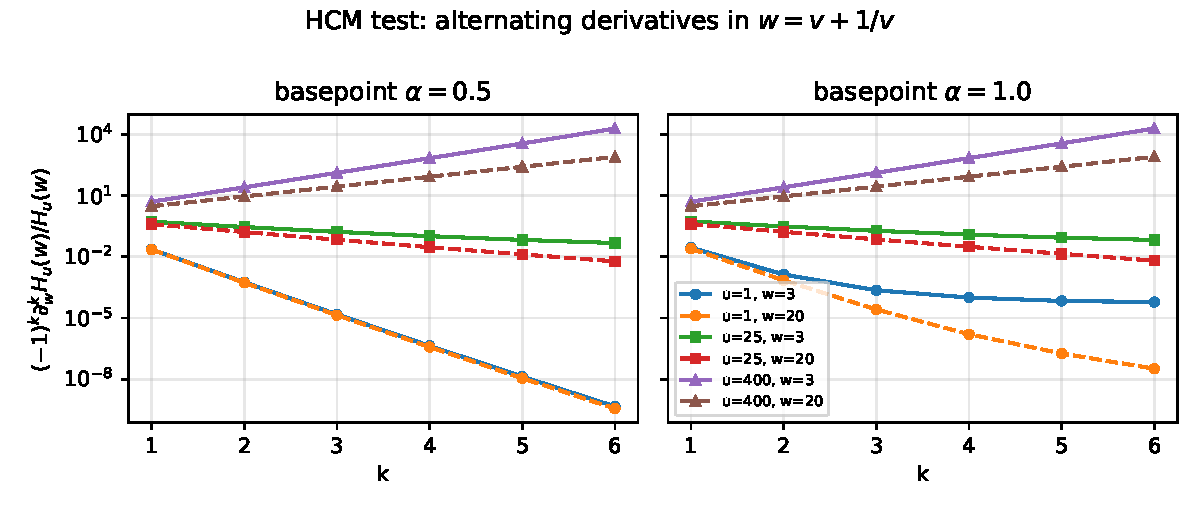
\includegraphics[width=0.95\textwidth]{fig/hcm.pdf}
\caption{Normalised alternating derivatives $(-1)^k\partial_w^kH_u(w)/H_u(w)$ of $H_u(w)=\varphi_\alpha(uv)\varphi_\alpha(u/v)$ for $1\le k\le6$, $u\in\{1,25,400\}$ and $w\in\{3,20\}$, computed from the P\'olya density, at the centre $\alpha=\tfrac12$ and at the unconditional basepoint $\alpha=1$. }
\label{fig:hcm}
\end{figure}
